We needed a way to intercept system and library calls made by an application in order to inject bad return values. The technique also needed to be difficult to detect, lest it be circumvented, and innocuous so that it would not disrupt the normal execution of the program apart from the return value given. Furthermore, it needed to be fine-grained enough so that only calls from the  application being tested would be intercepted, lest it crash our whole system.

\subsection{Library Interposition}
Using the environment variable \texttt{LD\_PRELOAD}, a user can specify a shared library object that is loaded before any others at dynamic linking time \cite{ldpreload}. Importantly, functions within this shared library take precedence over any other functions of the same name, even ones found in \texttt{libc} and other standard libraries.

\subsubsection{Benefits of LD\_PRELOAD}
\texttt{LD\_PRELOAD} affords several benefits to the amateur fuzz tester. Primarily, it is extremely simple to work with, and therefore difficult to get wrong: just set an environment variable and run the (dynamically linked) binary. We took this approach in order to test many calls and utilities as quickly as possible, but given more time we may have opted to use binary rewriting. Furthermore, this method enables the interception of calls many levels deep in the stack, even in other dynamically linked libraries. We perceive this to be a benefit, as programs that depend on shared libraries are taking on the risk that those libraries are written incorrectly.

\subsubsection{Limitations of LD\_PRELOAD}
There are several limitations to this method. Significantly, statically linked applications bypass our wrappers completely; however, we did not encounter any statically linked applications. Other approaches, such as the binary rewriting techniques used by Miller et al. \cite{bart} or a dynamic instrumentation tool such as DynInst \cite{dyninst}, circumvent this issue by modifying the binary directly, and would be necessary to expand coverage to statically linked programs.

Another limitation to our method is that it is Linux-specific. \texttt{LD\_PRELOAD} is found on many Linux distributions and some other UNIX systems, such as BSD \cite{bsd}. However, there are equivalents found on other popular systems such as the \texttt{AppInit\_DLLs} registry value on Windows \cite{dll} and the \texttt{DYLD\_INSERT\_LIBRARIES} environment variable on macOS \cite{macos}. Therefore, we feel confident that this methodology could find success when applied to applications on the most common commodity operating systems.

\subsubsection{Implementation}\label{ld_preload_implementation}
For each call of interest, we created a position-independent shared library object containing a single wrapper function with the name of the call. The wrapper simply returns an error value with probability $p$, or calls the real version of the function with probability $1-p$. In this way, we probabilistically either inject an error value, or allow the application to continue as usual. A visual representation of this mechanism is given in Figure \ref{fig:ld_preload}. Each program of interest was tested with one call being intercepted at a time.

This probabilistic approach is used to attempt to test all of the calls to a given function within an application. If error values were returned 100\% of the time, we would not be able to evaluate program behavior on all possible code paths. For example, if a program calls \texttt{malloc} in two locations and crashes or aborts after an error value is returned from the first, then the second call will never be reached. To account for different program structures, we tested each call for each program on a variety of error return probabilities, ranging from 1\% to 50\%. Applications that make a particular call many times require a lower probability of returning an error in order to cover all possible code paths. Likewise, applications that make a particular call (e.g. \texttt{fork}) infrequently require a higher probability of returning an error in order to cover all possible code paths.
\begin{figure}
  \centering
	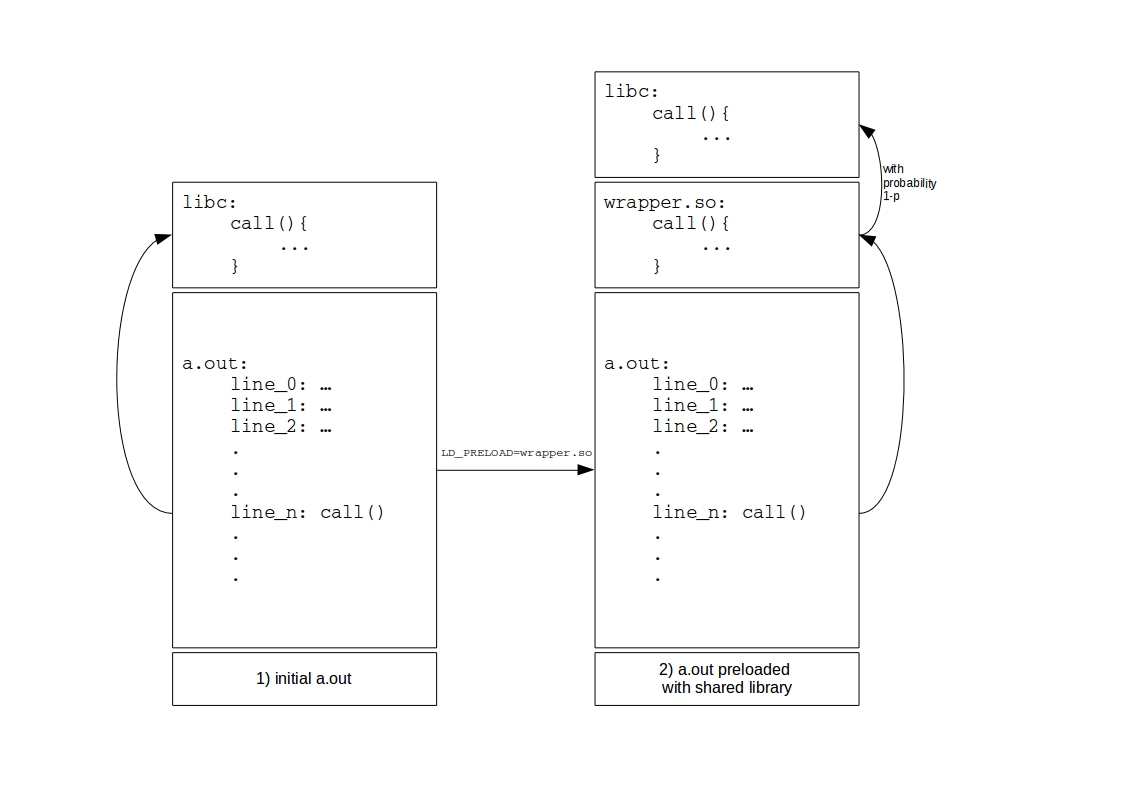
\includegraphics[width=0.8\textwidth]{ldpreload_fig}
	\caption{Library interposition allows for system and library calls to be overriden at runtime without recompilation or modification of the binary.}
  \label{fig:ld_preload}
\end{figure}

Returning the correct value from within a wrapped function is non-trivial: infinite recursion results if one attempts to invoke the same call that is being wrapped. To avoid the recursion, we used the \texttt{dlsym} function, which scans through the dynamically loaded libraries for a function that has the same name as the argument passed to it. Upon finding such a function, a function handle (that is, an address) is returned. This function handle can then be used in order to call the original version of the function. An example of such a wrapper is shown in the ``Generated Wrapper'' portion of Figure \ref{fig:codegen}.
